
%mainfile: Multimodal_learning.tex

\begin{titlepage}

  \centering

  \vspace*{1.5em}
  {\LARGE \scshape École Normale Supérieure \par}
  {\Large \scshape Département d'Informatique \par}

  {\Large \scshape Rapport de Stage de L3 \par}

  \vspace{14em}
  {\huge \bfseries Multimodal Learning \par} 
  {\Large \bfseries
    A case study for Gesture and Audio-Visual Speech Recognition \par}

  \vspace{4em}
  {\Large \scshape Hsieh Yu-Guan \par}
  
  \vspace{2em}
  {\Large Sous la direction de \par}

  \vspace{0.5em}
  {\Large \scshape Amélie Cordier$^1$ \& Mathieu Lefort$^2$ \par}

  \vspace{0.5em}
  {\large $^1$Hoomano, Équipe R\&D \par}
  {\large $^2$LIRIS, Équipe SMA \par}

  \vspace{8em}
  {\Large 14 Juin 2017 -- 11 Août 2017}

  \vfill

\end{titlepage}

\section{Introduction} \label{section:introduction}

\subsection{Cadre de travail, outils et environnement logiciel}

Mon stage s'inscrit dans le cadre du laboratoire commun BEHAVIORS.AI%
\footnote{\href{http://behaviors.ai/}{http://behaviors.ai/}}
qui est un projet de recherche collaboré entre la société Hoomano et LIRIS.
Hoomano est une entreprise créée en 2014 spécialisée dans le développement
de logiciel pour les robots sociaux (ex: Nao et Pepper).
Ils commercialisent un moteur d'interaction qui
vise à offrir une interaction homme-robot la plus naturelle possible.
Le LIRIS (Laboratoire en InfoRmatique, Image et Système d'Information)
est une unité mixte de recherche en informatique située à Lyon qui compte
14 équipes de recherche et 330 membres. Le laboratoire commun est
particulièrement lié à l'équipe SMA (Systèmes Multi-Agents) qui
met l'accent sur l'intelligence artificielle, les sysmèmes multi-agents,
et les systèmes cognitifs.

Pendant mon stage, j'ai passé les deux premières semaines au
laboratoire et pour le reste du temps j'étais à Hoomano car j'entraînais
les modèles sur le serveur de l'entreprise. Tous les codes ont été
réalisés en python et précisément à l'aide de la biblithèque open source
TensorFlow%
\footnote{\href{https://www.tensorflow.org/}{https://www.tensorflow.org/}}
développée par Google. Cela incluait la construction des
différents architectures et réseaux de neurones, l'entraînement et
l'évaluation.
TensorBoard était un outil assez pratique pour visualiser l'apprentissage,
et je pouvais même facilement visualiser les données et les
représentations apprises grâce au plugin qui est proposé.
Toute la suite du rapport sera rédigée en anglais à cause de la difficulté
de traduire tous les termes techniques en français.

\subsection{Scientific overview}

Historically, expert systems have been widely used for the design
of artificial intelligence. 
Agents rely heavily on handcrafted ontologies and symbolic rules to
make decisions and act in the world.
Although impressive results have been obtained with this line of
research, it requires a lot of engineering efforts and human knowledge.
Furthermore, engineering in this way all the behaviors that are needed
to display general human level intelligence is out of reach.

In addition, we face also the symbol grounding problem
\cite{S. Harnad 1990}. The symbols manipulated by the AI systems have
no meaning to them. To solve these problems, the embodied paradigm
\cite{A. Clark 1997} first argues an agent must be able to perceive and
act from its own perspective, so it should have a body, e.g. a robot.
Developmental robotics \cite{J. Weng 2001}, which draws inspiration
from developmental psychology \cite{J. Piaget 1952}, tries to implement
child development  in robots. It puts emphasis on the
importance of endowing the robot with the capacity of learning new
knowledge from its own sensorimotor experience.

In \cite{L. Smith 2005}, Smith and Gasser discerned six fundamental
principles for the development of embodied intelligence: multimodality,
incremental development, physical interaction with the environment,
exploration, social guidance and symbolic language acquisition.
I was particularly insterested in the multimodal point in my internship.
The everyday concepts that a human acquires is intrinsically multimodal.
For example, the word ``cat'' can be quickly associated with the visual
appearance of a cat, its vocalization, and the tactile feeling that
we have while petting a cat. The existence of neurons that receive
early information from different modalities have also been proven
\cite{S. Molholm 2002}.

In machine learning, recently, deep learning has achieved a great success in
various domains, such as image recognition \cite{A. Krizhevsky 2012},
text generation \cite{A. Graves 2013} or
machine translation \cite{I. Sutskever 2014}.
It has also been more and more often applied to multimodal inputs
\cite{J. Ngiam 2011, T. Baltrusaitis 2017}.
Its capacity of learning hierarchical representations of data in a
fully unsupervised way \cite{P. Vincent 2010, A. Radford 2015}
is particularly interesting in the domain of robotics.

In my internship, I studied mainly the application of multimodal learning
using deep networks in the fields of multimodal gesture recognition
and audio-visual speech recognition (AVSR).
I focused especially on the problem
of shared representation learning and knowledge transfer. I wanted to show
that the availablity of multiple modalities could enable the model
to learn a better representation for each single modality and that one can
leverage information from one modality to be used for another when there
is an imbalance of amount of data among different sources.

The report is organized as follows. In section \ref{section:related} I
briefly review related work on gesture recognition, AVSR and other
fields of multimodal learning.
In section \ref{section:networks}, I present
several basic deep neural network architectures playing an important
role in my work. In sections \ref{section:dataset} and
\ref{section:exp}, I describe respectively the datasets and common
experimental setups that were used in my internship. Experimental
details and results are given in sections \ref{section:uni} and
\ref{section:multi}. Finally, conclusions and perspectives are
presented in section \ref{section:conclusion}.

The source code of all of the work described here can be found on my
github: \href{https://github.com/cyber-meow/internship_2017}
{https://github.com/cyber-meow/internship\_2017}.

\section{Related Work} \label{section:related}

\subsection{Gesture recognition}

Gesture recognition has been studied for a while within the fields of
computer vision and pattern recognition
\cite{T. Starner 1998, S. Mitra 2007}.
Recently, deep learning algorithms have led to
significant advances in this domain \cite{M. Asadi-Aghbolaghi 2017}.
The use of Convolutional Neural Networks (CNNs, see \ref{subsection:CNN})
is the most common
\cite{J. Nagi 2011}. 3d CNNs are used to deal with image sequences in
\cite{P. Molchanov 2015}. Architectures that take multimodal inputs
have also grown in popularity. In \cite{N. Neverova 2013}
Neverova \textit{et al.} copes with color,
depth, skeleton and audio information using CNNs and Recurrent
Neural Networks (RNNs). Some other works use 3d CNNs and deep belief
networks (DBNs) while facing similar multimodal inputs
\cite{N. Neverova 2014, L. Pigou 2014, D. Wu 2016}.

\subsection{Audio-visual speech recognition (AVSR)}

AVSR is probably one of the earliest examples of multimodal research.
Most early works were based on various hidden Markov model (HMM) extensions
\cite{G. Potamianos 2004}, but the use of neural networks were also
explored \cite{C. Bregler 1994, B. P. Yuhas 1989}. 
In the past few years, AVSR has drawn attention from the
deep learning community
\cite{J. Ngiam 2011, K. Noda 2014, A. K. Katsaggelos 2015}.
In \cite{J. Ngiam 2011} the authors use a deep network to learn a
joint representation of visual and auditory input.
They show that better features for one modality can be learned if
multiple modalities are present at feature learning time.
A transfer deep learning framework applied in AVSR is proposed in
\cite{S. Moon 2015} and this forms the base of my study in
\ref{subsection:AVSR_transfer}. In \cite{L. Deng 2013} and
\cite{G. Hinton 2012} several examples of how deep architectures can
be used to deal with audio data are given.

\subsection{Multimodal learning in other fields}

Multimodal learning also finds its application in many other domains.
For example, there has been a surge of interest in the exploitation of
multimodal
information in the fields of image annotation \cite{J. Weston 2010},
zero-shot learning \cite{A. Frome 2013, R. Socher 2013}, and automatic
image caption generation \cite{A. Karpathy 2015}. They first train
visual and language models separately and as a next step they try
to learn either a common embedding \cite{J. Weston 2010}, a mapping
\cite{A. Frome 2013, R. Socher 2013} or an alignment \cite{A. Karpathy 2015}
between the two models.

More generally, in \cite{T. Baltrusaitis 2017} Baltrusairis \textit{et al.}
offer an overview of recent advances in multimodal machine learning.
They identify five core technical challenges surrounding this research
field: shared representation learning, translation from one modality to
another, multimodal alignment that aims to
find correspondences between sub-components of instances from two
or more modalities, multimodal fusion that integrates information
from multiple modalities with the goal of predicting an outcome measure
and co-learning which aids the modeling of a modality by exploiting
knowledge from another modality.

Concerning the use of multimodal learning in robotics, in 
\cite{A. Droniou 2014} Droniou \textit{et al.} propose a network that is
able to learn both
a symbolic representation of data and a fine discrimination between
two similar stimuli in an unsupervised way. The authors apply their method
to visual, auditory and proprioceptive data of the humanoid robot iCub.
A multimodal embedding that is able to combine information coming from
vision, language and motion trajectories is defined in \cite{J. Sung 2017}
and endows the robot with the capacity of manipulating an unseen object.

\section{Presentation of Some Deep Network Architectures}
\label{section:networks}

\subsection{Convolutional Neural Networks} \label{subsection:CNN}

CNNs are an early family of deep learning
architectures inspired from the human vision system \cite{Y. LeCun 1998}.
Generally we have convolutional layers alternating with pooling
(subsamping) layers, but fully connected layers can also be introduced
(see \autoref{fig:CNN10}).
CNNs have been shown to achieve state-of-the-art performance in
image processing tasks such as image classification
\cite{A. Krizhevsky 2012} and object detection \cite{Y. LeCun 2010}.
However they can be equally applied in other fields like speech recogntion
\cite{L. Deng 2013}.

For a convolutional layer with a mono-channel input $x$, the latent
representation of the k-th feature map is given by

\[h^k = \sigma(x\ast W^k + b^k)\]

where $W^k$ is the k-th kernel, $b^k$ the bias is broadcasted to the whole
feature map, $\ast$ denotes the 2d convolution and $\sigma$ is an
ativation function.
Currently, ReLu (Rectified Linear Units) is probably the one that is the
most commonly used for a CNN \cite{A. Krizhevsky 2012}.
It is defined by

\[\sigma(x) = x^+ = max(0,x),\]

when $x$ is a single scalar and otherwise the above function is applied
to each element of the input.
The convolution kernel is extended to the full depth of input when there
are multiple input channels.
On the contrary, no parameters are required for defining a pooling layer.
It just take some $d \times d$ region (supposing that the kernel has the
same height and width) and output a single value, which for example,
is the maximum in that region when using max-pooling.

There are yet two other important factors that are used to define these
operations: \textit{stride} and \textit{padding}.%
\footnote{Due to the space limit, more details of the CNN architecture,
including the role of these two hyperparameters, can be found here:
\href{http://cs231n.github.io/convolutional-networks/}
{http://cs231n.github.io/convolutional-networks/}.}
Concerning this, two different zero paddings are defined in TensorFlow,
`SAME' and `VALID'. For `SAME' padding, $h_o = \lceil h_i/s_h \rceil$,
and for `VALID' padding, $h_o = \lceil (h_i-h_f+1)/s_h \rceil$,
where $h_i$, $h_o$, $h_f$ are respectivly the height of the input
feature map, the output feature map and the filter (kernel) and
$s_h$ is the stride of the height
dimension. Similar formulas also exist for the width.%
\footnote{
\href{https://www.tensorflow.org/api\_guides/python/nn\#Convolution}
{https://www.tensorflow.org/api\_guides/python/nn\#Convolution}.}

Suppose all the parameters of a CNN model have been learned, the model
is then ready to be used for a specific task. One just needs to run the
model forward as decribed above. Therefore, the purpose of the learning
phase is to find the appropriate parameters that can help us solve the task.
Mathematically, this is achieved by optimizing the weights of the network
to minimize some loss function (e.g. cross entropy
or L2 distance, see section \ref{section:exp}).
The optimization is usually done by a SGD-based algorithm.
SGD is the abbreviation of stochastic gradient descent. At each
training step, we compute the gradients of the loss with respect to all
weights in the network and then update the weights according to these
gradients. Using the chain rule, gradients are computed layer by
layer (starting from the output of the network) and the error is thus
\textit{back-propagated} to the whole network.%
\footnote{
\href{http://andrew.gibiansky.com/blog/machine-learning/convolutional-neural-networks/}
{http://andrew.gibiansky.com/blog/machine-learning/convolutional-neural-networks/}.}

In \cite{S. Ji 2013}, 3d CNNs are proposed to be used for video inputs.
They're like traditional CNNs except for the fact that we replace
2d feature maps by 3d feature maps and 2d kernels by 3d kernels.

\subsection{Auto-Encoder} \label{subsection:AE}

Auto-Encoders are networks that are trained to minimize the reconstruction
error by back-propagating it from the output layer to hidden layers.
In the simplest model with one hidden layer, an auto-encoder takes an
input $\mathbf{x} \in \mathbb{R}^d$ and maps it to the latent
representation $\mathbf{h} \in \mathbb{R}^{d'}$ given by
$\mathbf{h} = \sigma(W\mathbf{x}+\mathbf{b})$ where $W$
is a weight matrix, $\mathbf{b}$ is a bias vector and $\sigma$ is an
activation function. Then the network tries to reconstruct the input
by a reverse mapping $\mathbf{x'} = \sigma(W'\mathbf{h}+\mathbf{b'})$.
The loss function can be for instance $||x' - x||$ where $||.||$ is
some distance.

To prevent the auto-encoder from learning the identity function as
a trivial solution, several regularization techniques have been proposed.
The bottleneck approach forces dimensionality reduction by having
fewer neurons in hidden layers than in the input layer. For example,
in the above case, we must have $d'<d$. Sparse auto-encoders impose sparsity
on hidden units \cite{A. Makhzani 2014}.
Denoising auto-encoders, which played an important role in my work,
try to recontruct the clean input from its corrupted version
\cite{P. Vincent 2008, Y. Bengio 2012}. Binomial noise
(switching pixels on or off) adding
to input or hidden layers were used in my case.

Intuitively, auto-encoders are useful for data reconstruction.
Nevertheless, the true interest lies in fact in its capacity to learn
a representation (encoding) for a set of data in a purely unsupervised
fashion \cite{P. Vincent 2010}. Recently, auto-encoders have also
been more and more used as a generative model \cite{Y. Bengio 2013}.

\subsection{Convolutional Auto-Encoder}

Fully connected auto-encoders ignore the 2d image structure.
This can cause problems when dealing with real-world size inputs,
and introduce redundancy in the parameters.
Convolutional Auto-Encoders \cite{J. Masci 2011, V. Turchenko 2017}
(CAEs) are intuitively similar
to architectures described in \ref{subsection:AE}.
However, convolutional and transposed convolutional layers are used instead.
Transposed convolutional layers are also called deconvolutional
layers \cite{M. D. Zeiler 2011}.
We perform in fact also a convolution operation but with zero paddings
around the image and sometimes around each pixel to upsample the
image and to inverse the previous convolution
(imagine that if the value of one pixel comes from 9 pixels of the
previous layer, when doing a transposed convolution this pixel
contributes to the same 9 pixels for reconstruction).
This github directory
\href{https://github.com/vdumoulin/conv_arithmetic}
{https://github.com/vdumoulin/conv\_arithmetic}
is quite useful for the understanding of the concept.

Pooling and unpooling layers are also sometimes considered in a CAE
architecture \cite{V. Turchenko 2017}.
More details on this aspect, which was not used in my work, can be found in
in \cite{H. Noh 2015, V. Turchenko 2017}.

\vspace{-1em}
\begin{figure}[H]
  \centering
  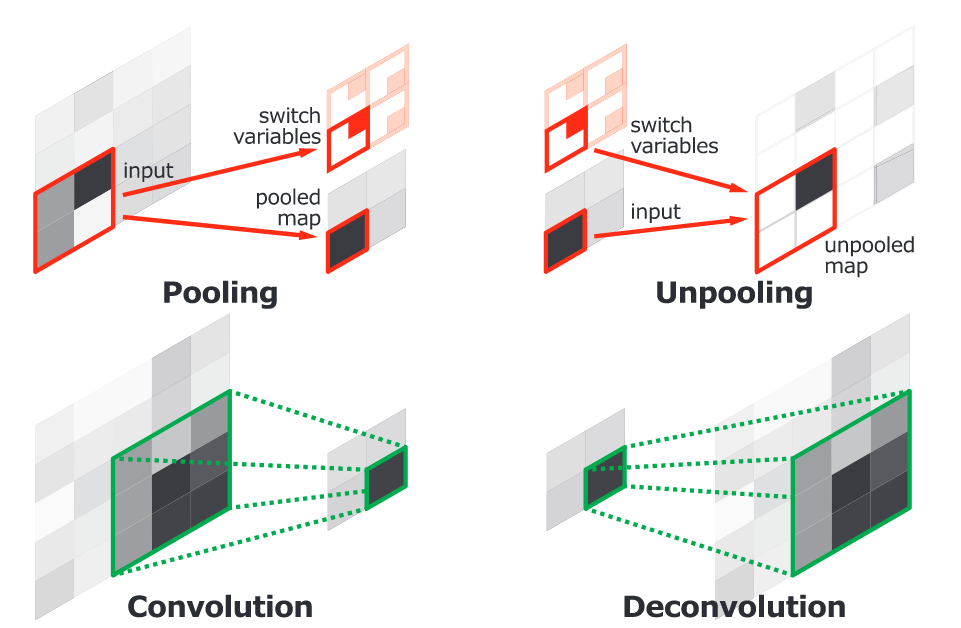
\includegraphics[width=0.5\linewidth]{architectures/layers}
  \caption{%
    \textbf{Illustration of deconvolution and unpooling layers
      \cite{H. Noh 2015}}}
  \label{fig:layers}
\end{figure}

\section{Datasets and Preprocessing} \label{section:dataset}

Many datasets were explored during my internship. In this report,
I will only detailed the three that I used the most. Two of them are for
gesture recognition: Creative Senz3D \cite{A. Memo 2015, A. Memo 2017}
and ASL Finger Spelling \cite{N. Pugeault 2011}, and one is for AVSR:
AVLetters \cite{I. Matthews 2002}.

\subsection{Creative Senz3D}

The dataset contains gestures coming from 4 different people, each
performing 11 different static gestures repeated 30 times each,
for a total of 1320 samples.
For each sample, color, depth and confidence frames are available.
I only used the color and depth frames of this dataset since my
architectures take at most two modalities in input. The original
size of each image is $480 \times 640$ and they're resized to
$299 \times 299$ pixels before being fed to the network since this
is also the input size of the Inception model \cite{C. Szegedy 2017}.
No other preprocessing are done. For both color and depth images I use
the three color channels (even though a priori only one channel is needed
for depth maps).

\begin{figure}[H]
  \centering
  \hfill
  %
  \begin{subfigure}{0.23\linewidth}
    \centering
    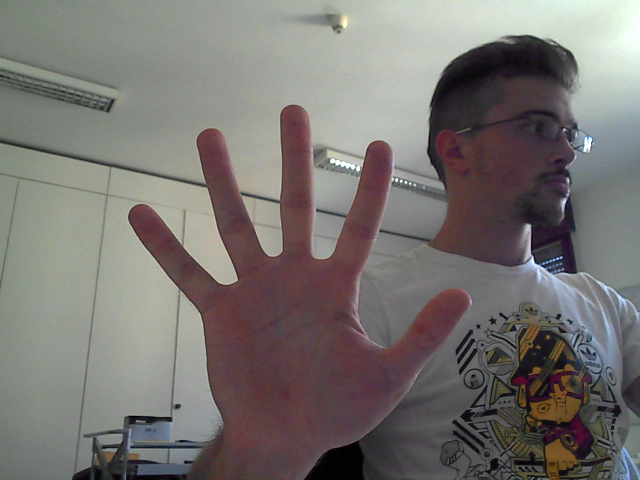
\includegraphics[width=\textwidth]{dataset/senz3d/examples/1-color}
    \caption{}
  \end{subfigure}
  %
  \hfill
  %
  \begin{subfigure}{0.23\linewidth}
    \centering
    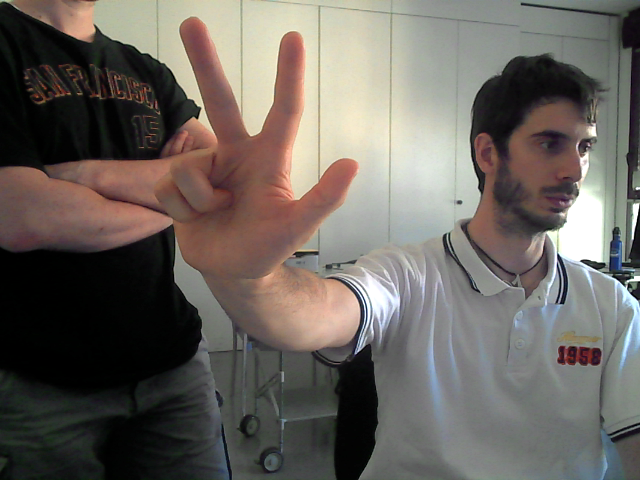
\includegraphics[width=\textwidth]{dataset/senz3d/examples/12-color}
    \caption{}
  \end{subfigure}
  %
  \hfill
  %
  \begin{subfigure}{0.23\linewidth}
    \centering
    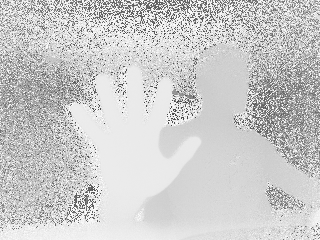
\includegraphics[width=\textwidth]{dataset/senz3d/examples/1-depth}
    \caption{}
  \end{subfigure}
  %
  \hfill
  %
  \begin{subfigure}{0.23\linewidth}
    \centering
    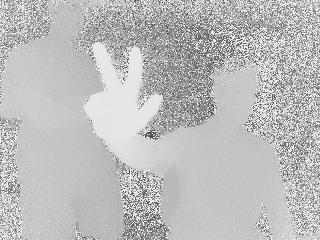
\includegraphics[width=\textwidth]{dataset/senz3d/examples/12-depth}
    \caption{}
  \end{subfigure}
  %
  \caption{%
    \textbf{Example images in the Creative Senz3D dataset.}\\[0.1em]
    a, b) Color images.\\[0.1em]
    c, d) Corresponding depth images. (c) and (d) are respectively the
      depth images of (a) and (b).\\[0.1em]
    All of the images are of size $480 \times 640$ and contain the
      the entire upper body of the subject.}
  \label{fig:senz3d_exs}
\end{figure}

\subsection{ASL Finger Spelling}

The dataset is composed of more than 60000 images in each modality
(RGB and depth images are provided).
Five subjects are asked to perform the 24 static signs in
the American Sign Language (ASL) alphabet (excluding j and z which involve
motion) a certain number of times, captured with similar lighting
and background.

Images of this dataset are of variable sizes. The data preprocessing
includes resizing each image to $83 \times 83$ pixels,
converting them to grayscale and Z-normalization (normalizing to zero mean
and unit of variance).

\begin{figure}[H]
  \centering
  \hfill
  %
  \begin{subfigure}{0.21\linewidth}
    \centering
    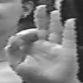
\includegraphics[width=\linewidth]{%
      dataset/fingerspelling5/exs/st/g1}
    \caption{}
  \end{subfigure}
  %
  \hfill
  %
  \begin{subfigure}{0.21\linewidth}
    \centering
    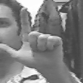
\includegraphics[width=\linewidth]{%
      dataset/fingerspelling5/exs/st/g2}
    \caption{}
  \end{subfigure}
  %
  \hfill
  %
  \begin{subfigure}{0.21\linewidth}
    \centering
    
\includegraphics[width=\linewidth]{%
      dataset/fingerspelling5/exs/st/d1}
    \caption{}
  \end{subfigure}
  %
  \hfill
  %
  \begin{subfigure}{0.21\linewidth}
    \centering
    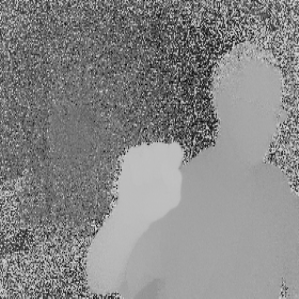
\includegraphics[width=\linewidth]{%
      dataset/fingerspelling5/exs/st/d2}
    \caption{}
  \end{subfigure}
  %
  \caption{%
    \textbf{Example images in the ASL Finger Spelling dataset
      (after preprocessing).}\\[0.1em]
    a, b) Grayscale intensity images.\\[0.1em]
    c, d) The corresponding depth maps. (c) and (d) are respectively the
      depth images of (a) and (b).\\[0.1em]
    Images of this dataset have variable sizes, and they're all resized to
      $83 \times 83$ before being fed to the network. Generally only the
      hand region is contained in the image.}
  \label{fig:fingerspelling_exs}
\end{figure}

\subsection{AVLetters}

The dataset comprises video and audio recordings of 10 speakers
uttering the letters A to Z, three times each.
We count therefore 780 samples in total. For video data, image sequences
of pre-extracted lip regions are provided.
Each single image is of size $60 \times 80$.
For audio data, only the mel-frequency cepstrum coefficients (MFCCs%
\footnote{MFCCs are a feature widely used in automatic speech and
speaker recognition. Their job is to extract spectral envelope
in order to discriminate the phoneme being pronounced.})
are given, and each audio frame is represented by 26 MFCCs.
The lack of raw audio data is a strong constraint on what we're able to do
on this dataset.

Since all utterances do not have the same time duration, I used
fourier resampling to force every video input to be of length 12 and
every audio input to be of length 24. These numbers were chosen according
to \cite{S. Moon 2015}. Video frames are Z-normalized.
Several data augmentation techniques are also considered, including
random brightness adjusting, random contrast adjusting and random
cropping (but at least 80\% of the original image is kept).
The data is augmented on the fly.

\begin{figure}[H]
  \centering
  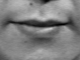
\includegraphics[width=0.15\linewidth]{%
    dataset/avletters/lips_no_data_aug/1}
  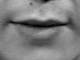
\includegraphics[width=0.15\linewidth]{%
    dataset/avletters/lips_no_data_aug/2}
  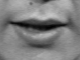
\includegraphics[width=0.15\linewidth]{%
    dataset/avletters/lips_no_data_aug/3}
  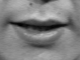
\includegraphics[width=0.15\linewidth]{%
    dataset/avletters/lips_no_data_aug/4}
  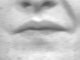
\includegraphics[width=0.15\linewidth]{%
    dataset/avletters/lips_no_data_aug/5}
  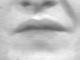
\includegraphics[width=0.15\linewidth]{%
    dataset/avletters/lips_no_data_aug/6}\\[0.15em]
  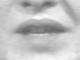
\includegraphics[width=0.15\linewidth]{%
    dataset/avletters/lips_no_data_aug/7}
  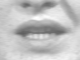
\includegraphics[width=0.15\linewidth]{%
    dataset/avletters/lips_no_data_aug/8}
  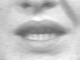
\includegraphics[width=0.15\linewidth]{%
    dataset/avletters/lips_no_data_aug/9}
  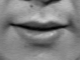
\includegraphics[width=0.15\linewidth]{%
    dataset/avletters/lips_no_data_aug/10}
  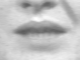
\includegraphics[width=0.15\linewidth]{%
    dataset/avletters/lips_no_data_aug/11}
  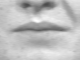
\includegraphics[width=0.15\linewidth]{%
    dataset/avletters/lips_no_data_aug/12}
  \caption{%
    \textbf{Example visual input for the AVletters dataset.}\\[0.1em]
    Pre-extracted lip regions of $60 \times 80$ pixels are provided.
      Each image sequence is resampled to be of length twelve in order to
      give an input of fixed size to the network. In the above figure,
      time goes from left to right then top to bottom.}
  \label{fig:avletters_exs}
\end{figure}

\section{Experimental Setup} \label{section:exp}

Each classifier used in my work was trained with the cross entropy cost
function and each auto-encoder was trained with the L2 distance between
the input and output vector was used as the loss.
The cross entropy measures the similarity between two probability
distributions $p$ and $q$ over the same underlying set of events.
When $p$ and $q$ are disrcret, which is always true in my case, it's
defined by

\[H(p,q) = -\sum_xp(x)\log q(x).\]

For the sake of preventing overfitting, L2
regularization \cite{Y. Bengio 2012} was applied to all the weights of
network with a regularization coefficient $\lambda$.
The Adam algorithm \cite{D. Kingma 2014}, which is a variant of the
standard SGD, was then introduced for minimizing the loss function.
An exponential decay was further used for the stepsize $\alpha$ of this
algorithm with an initial stepsize $\alpha_0$ varying from 0.01 to 0.0001
depending on experiment. The decaying rate $\gamma$
was generally close to 0.8 and the decay takes place every 100
training steps. That is, the stepsize is multiplied by $\gamma$ every
100 steps.

Inputs of the network were normally fed as mini-batches of size 24
since rather satisfying results could be obtained with this
number and when larger batches were used training became slower
without a significant improvement of the performance.
Batch normalization \cite{S. Ioffe 2015} were introduced after every
convolutional and transposed convolutional layer. Therefore, the real
operations used to compute neural activations are more complicated
than what are described above. The presented settings and hyperparameter
values were found with a manual heuristic search as I focused on
principles and not on better performance achievement.

Here are some more details of the network architectures: ReLu activations 
were added to all the hidden layers of all the architectures
\cite{A. Krizhevsky 2012} while no activation function was used for
the output layers.
For classification model dropout \cite{N. Srivastava 2014}
was always applied to the second to last layer during training.
The output of the classification layer was mapped to the probabilities
that one data example belongs to each class by the softmax function.
Therefore, if the output vector is $\mathbf{z} = (z_1, ..., z_n)$,
for $j \in \{1,...,n\}$, the probability that the input has the $j^{th}$
label is

\[softmax(\mathbf{z})_j = \frac{\exp(z_j)}{\sum_{i=1}^n\exp(z_i)}.\]

For classification experiments, except for the one described in
\ref{subsection:AVSR_transfer}, the dataset was always separated into
training and test set. The classifier was first trained on the training data
and then tested on test data once the training phrase was finished.
Unless stated otherwise, the prediction accuracies mentioned hereinafter
were always evaluated on the test set.

Moreover, we can consider two different possible settings:\\[0.25em]
\textbf{Subject Dependent.}
In a subject dependant setting, data samples are separated randomly into
training set and test set. Therefore, during the
testing phase, the classifier does not need to deal with data from an
individual that it has never seen before.\\[0.25em]
\textbf{Subject Independant.}
On the contrary, the classifier faces individuals never seen before
during testing in a subject independant setting. 
In my case, I always separated one subject from the others to form
the test set while the training set consisted of the rest of the data.

\section{Experiments and Results: Unimodal Cases} \label{section:uni}

\subsection{Classification} \label{subsection:classif}

For every dataset, I began with training a classifier on it in a
totoally supervised manner.
This gave me an insight into its data quality, the preprocessing
effectiveness and ensured that further experiments could be conducted.
CNN is then one of the most suitable architecture for this purpose.

First, it's worth mentioning the problem of overfitting.
It was observed for almost all the classification experiments that I
carried out, and it was particularly severe for CNNs with many layers.
In fact, CNN architectures could usually classify
perfectly the training data, but experienced a drop of performance
when evaluating on test set.

It is well known that by reducing the number of hidden layers and
increasing the weight regularization coefficient $\lambda$ we may
be able to cure this problem.
For example, when $\lambda$ was augmented from $0.0004$ to $0.1$,
the classification accuracy for the audio input of the AVLetters
dataset increased by about 10 points
(from 63.22\% to 77.84\%) while using the architecture detailed on
the left side of \autoref{fig:AVSR_transfer} with the hyperparameters
given in \autoref{tab:AVSR_transfer}.
By using fewer hidden layers in the 3d CNN architecture overfitting
was also alleviated when dealing with the video input of this same dataset.
However, these techniques did not always work
and more often I got a poorer performance during training without
an improvement of performance for test.

Below I'll briefly describe the final results of this part dataset by
dataset.

\subsubsection{Creative Senz3d}

The tested architectures were perceptron (in all of this report by
perceptron I denote a single-layer perceptron), pre-trained InceptionV4
model \cite{C. Szegedy 2017} and several hand-coded CNNs%
\footnote{For those who are interested, please refer to my github
directory for the used hyperparameters.}.
The lack of data quantity, variety, and the fact that the head is also
contained in the image seems to increase the classification difficulty.
In conlusion, I found that it was more interesting to use a subject
dependent setting for this dataset. In this case, for RGB images,
all of the classifiers were able to have a classification accuracy that is
closed to 100\%. For depth images, the classification accuracy was
between 60\% and 70\% using a perceptron and near 90\% for other
architectures.

\subsubsection{ASL Finger Spelling} \label{subsubsection:ASL_CNN}

The large number of data contained in this dataset and the relatively
simple image content (single hand instead of the entire upper body)
makes the classification task much easier. By using the CNN architecture
shown in \autoref{fig:CNN10}, I could achieve a classification accuracy
of respectively 79.73\% and 64.46\% for intensity and depth images
(see \autoref{tab:ASL_classif})
in a subject independant setting (four subjects for training and one
subject for testing). Fewer layers in the CNN architecture may also allow
us to achieve the same performance. More experiments need to be carried
out to find the most suitable hyperparameters.

\vspace{-1em}
\begin{figure}[H]
  \centering
  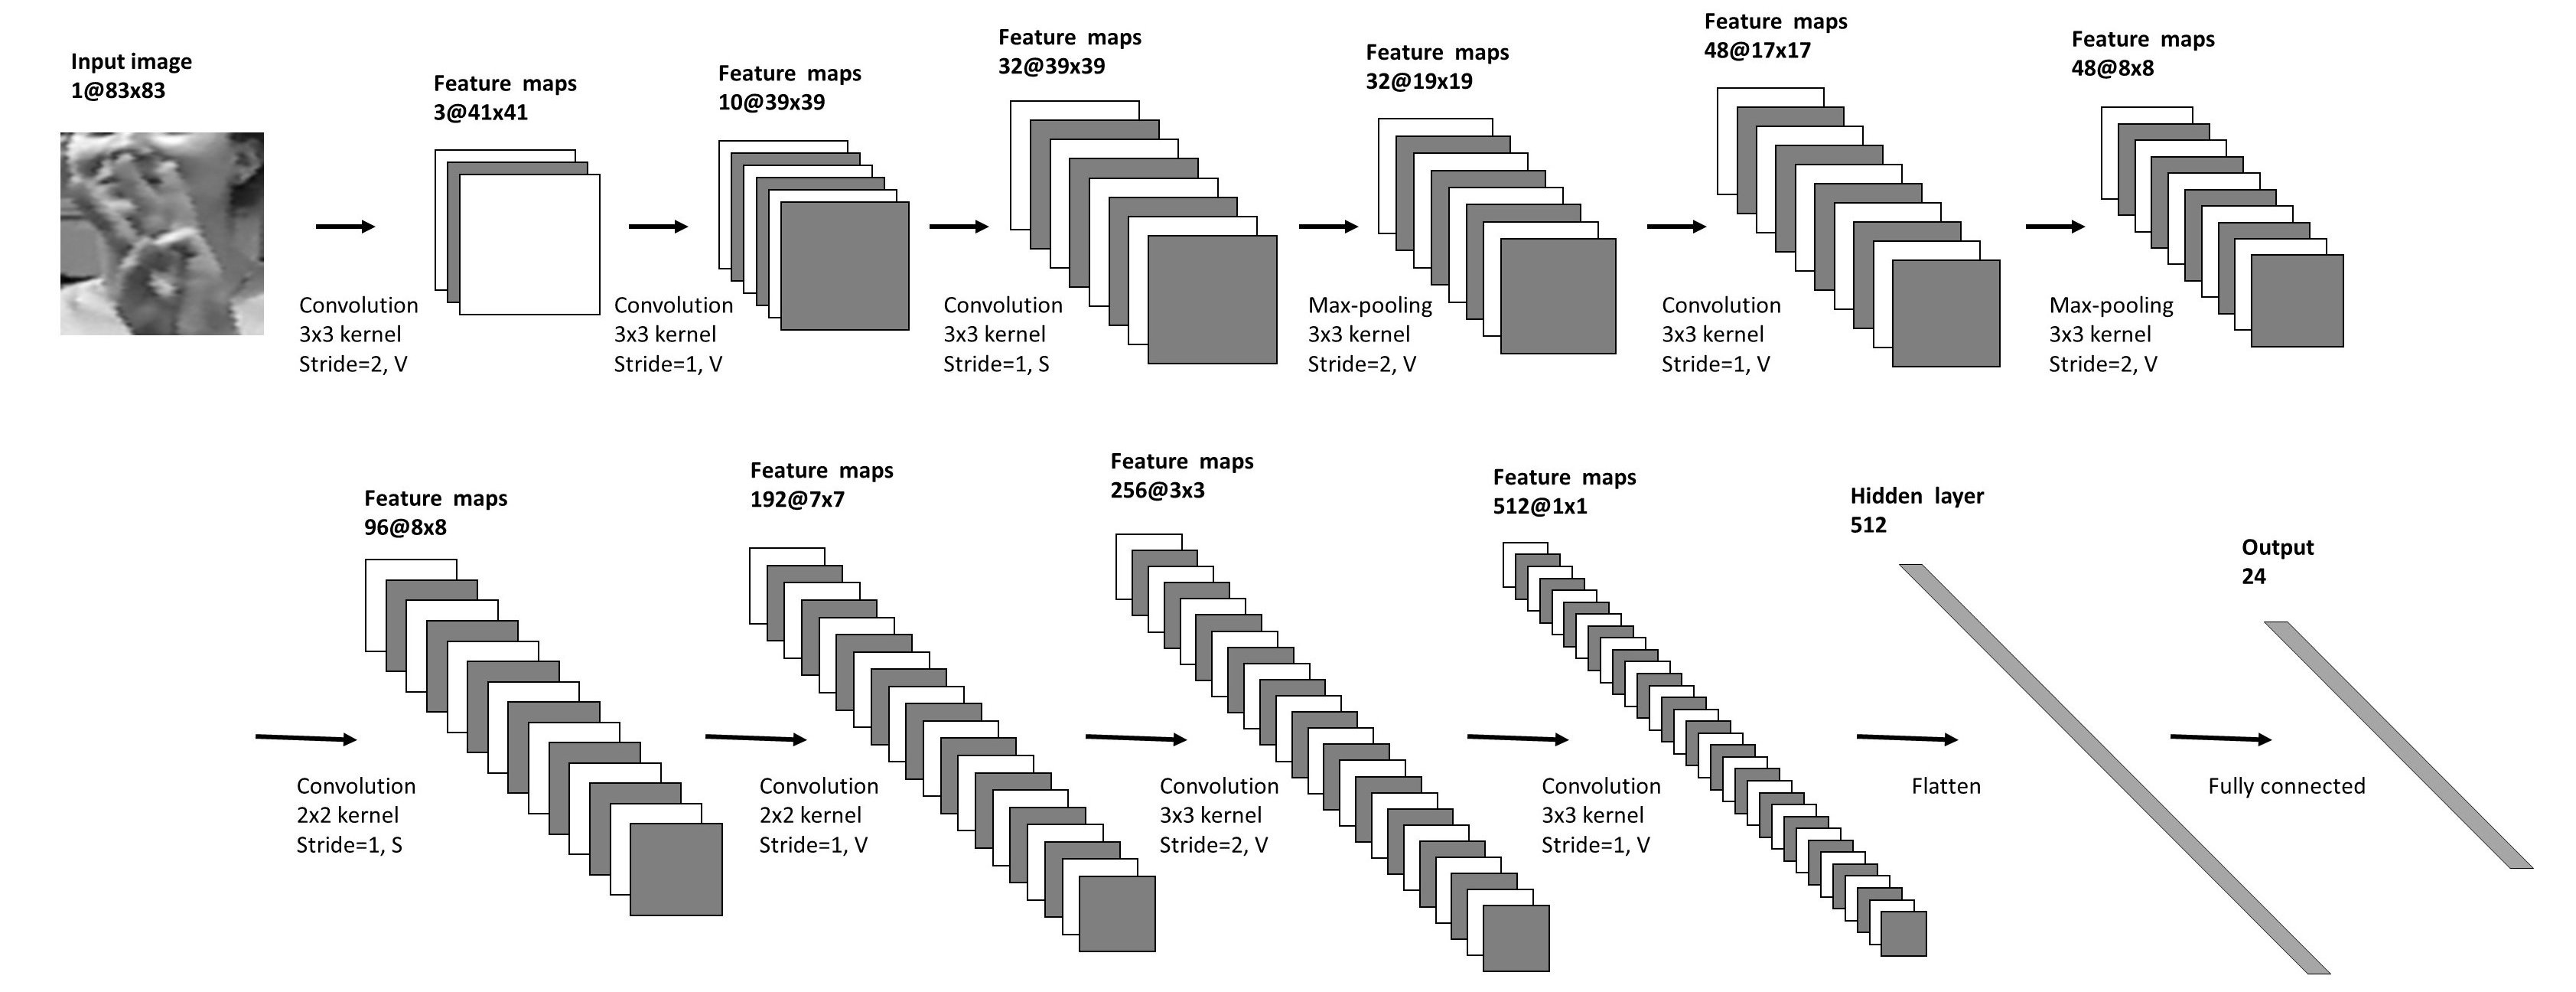
\includegraphics[width=\linewidth]{architectures/CNN10}
  \caption{%
    \textbf{CNN architecture used for the Finger Spelling  dataset.}
      \\[0.1em]
    The input of the nework is a one-channel image of size $83 \times 83$.
      It contains ten hidden layers. S stands for `SAME' padding
      and V stands for `VALID' padding (see \ref{subsection:CNN}).}
  \label{fig:CNN10}
\end{figure}

\subsubsection{AVLetters}

One can refer to \autoref{fig:AVSR_transfer} for the main CNN architectures
that were used in this dataset. 
Notice that 3d CNNs were employed to deal with video inputs.
Considering the small number of available data, a speaker dependent
setting was used.
With some carefully chosen hyperparameter values and network architectures
(see \autoref{fig:AVSR_transfer} and \autoref{tab:AVSR_transfer}),
the prediction accracy was of 77.84\% for audio and 54.32\% for video.

\subsection{Convolutional auto-encoder} \label{subsection:CAE}

Several distinct CAE hyperparameters were tested during my internship.
Here I present the one with five hidden layers; therefore it contains
three convolutional layers and three transposed convolutional layers
as illustrated in \autoref{fig:CAE5}. I used end-to-end training for
learning my architectures.

The proposed architecture was then trained on the two gesture recognition
datasets. First of all, I was interested in the denoising capcity of
the auto-encoder. An example is given in \autoref{fig:image_restoration}.
The auto-encoder is effectively able to reconstruct the clean image in
a way, even though the result is blurred and sometimes distorted.

What's more important, can meaningful high-level features be
learned in this way? 
In fact, when autonomous robots interact with the environment, it needs
to extract high-level knowledge from raw perception on its own.
This should be done in an unsupervised way since no labeled data
is provided.
That is why I am particularly interested in the problem of representation
learning here. The output of the middle layer was taken as a new
representation of the input data.
I wanted to show that it could better represent the data than the raw input.

By doing principal component analysis, activation values of different
layers could be projected into three dimensions for visualization.
However, to quantify the learned features, I further trained two perceptrons
respectively on top of the raw input and the high-level representation
and compared their performance.

As suggested in \ref{subsection:classif}, I used a subject dependant setting
for Creative Senz3d while a subject independant setting was employed
for ASL Finger Spelling. As already mentioned earlier, a perceptron built
on raw data could classify perfectly the input while dealing with color
images of Creative Senz3d. In other cases, the use of the learned
data representation led always to an improvement of 10-20 points for
the prediction accuracy (refer to \autoref{tab:ASL_classif}
for results on ASL Finger Spelling). Useful high-level data representation
can thus be learned in a totally unsupervised manner.
However, if this same architecture used for classification (three layers
of convolution and one layer of classification) was trained in a
totally supervised manner, this was as if I trained another CNN and
better performance could be achieved (see the column CAE architecture
of \autoref{tab:ASL_classif}).

\vspace{-1em}
\begin{figure}[H]
  \centering
  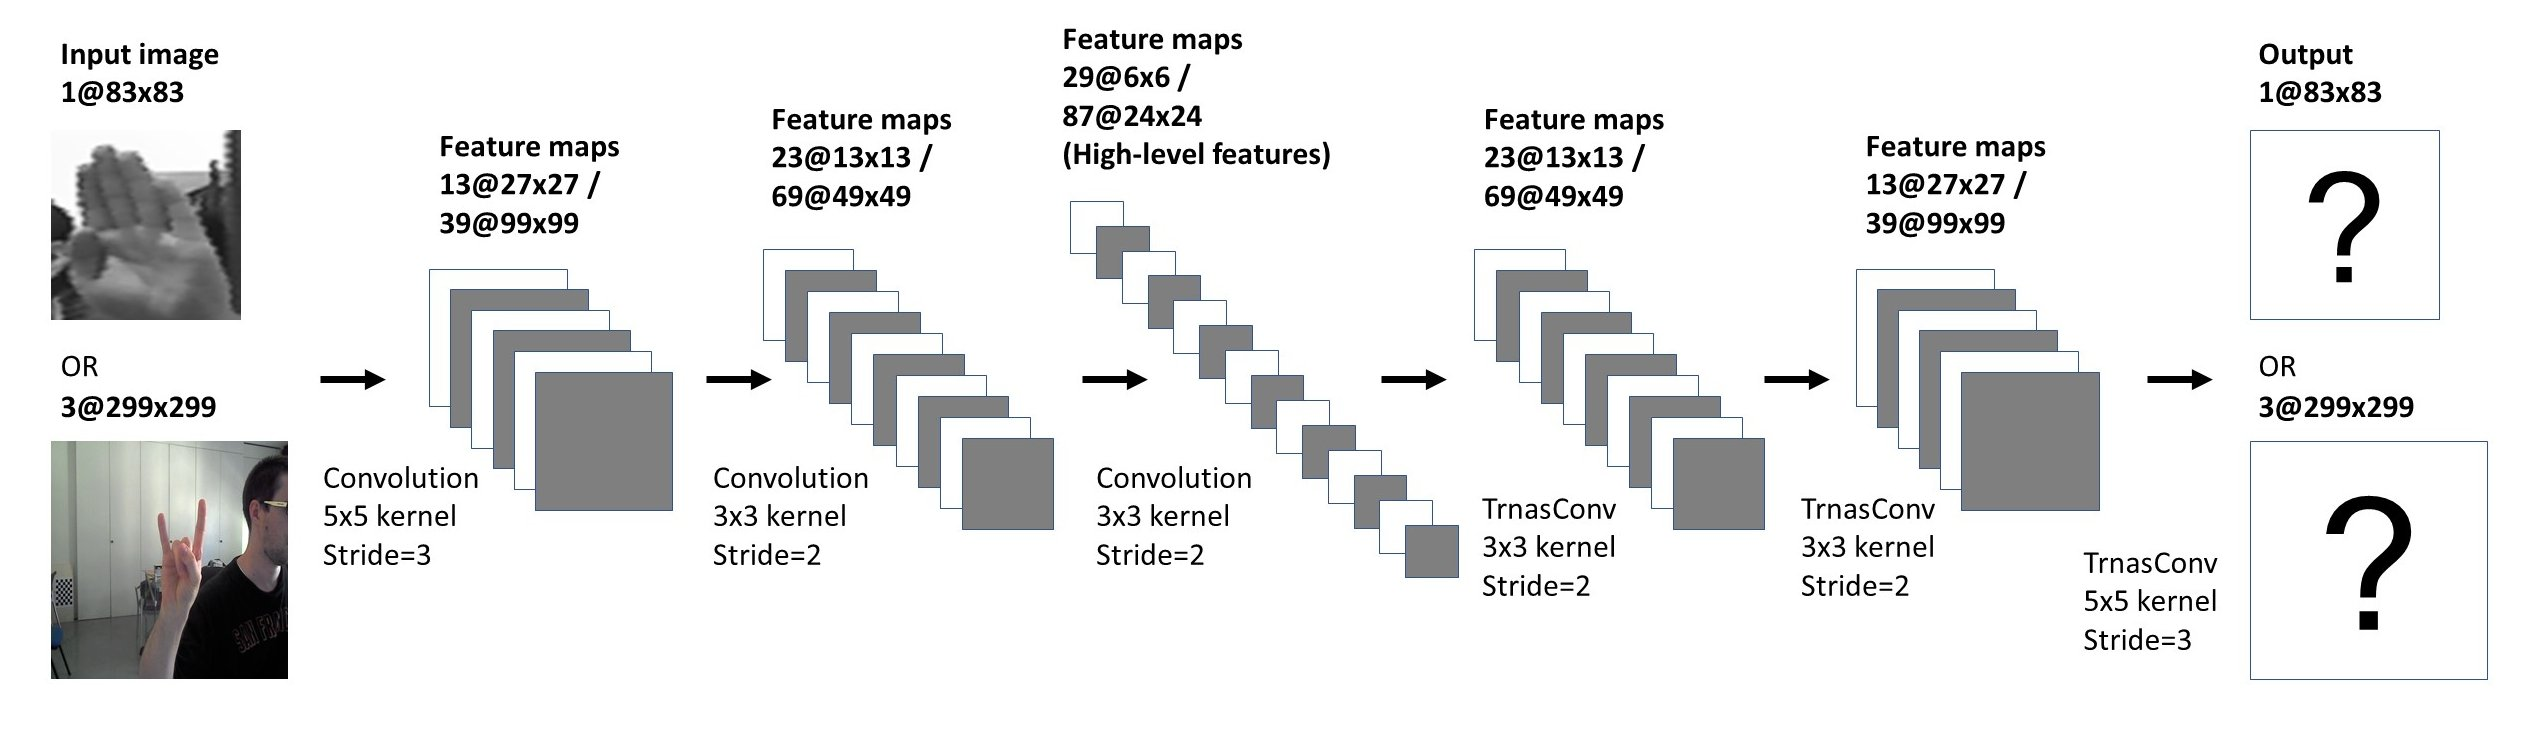
\includegraphics[width=\linewidth]{architectures/CAE5}
  \caption{%
    \textbf{Convolutional auto-encoder architecture with 
      three convolutional layers and three tranposed convolutional
      layers.}\\[0.1em]
    Activation values of the middle layer are taken as 
      high-level features of the input image. Inputs of the network
      can be of different sizes. We only use `VALID' paddings here.
      For the results that are presented in this work, the training
      hyperparameters are $\alpha_0 = 0.01$, $\gamma = 0.8$ and
      $\lambda = 0.0004$ (see the first paragraph of section
      \ref{section:exp}).
      }
  \label{fig:CAE5}
\end{figure}

\begin{figure}[H]
  \centering
  \hfill
  %
  \begin{subfigure}{0.28\linewidth}
    \centering
    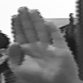
\includegraphics[width=\linewidth]{%
      dataset/fingerspelling5/gray/gray5}
    \caption{}
  \end{subfigure}
  %
  \hfill
  %
  \begin{subfigure}{0.28\linewidth}
    \centering
    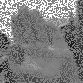
\includegraphics[width=\linewidth]{%
      dataset/fingerspelling5/gray/gray_dropout5}
    \caption{}
  \end{subfigure}
  %
  \hfill
  %
  \begin{subfigure}{0.28\linewidth}
    \centering
    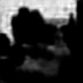
\includegraphics[width=\linewidth]{%
      dataset/fingerspelling5/gray/gray_reconstruction5}
    \caption{}
  \end{subfigure}
  %
  \caption{%
    \textbf{Image restoration using convolutional auto-encoder.}\\[0.1em]
      a) Clean Image.\\[0.1em]
      b) Noisy image [input].\\[0.1em]
      c) Restored image [output].}
  \label{fig:image_restoration}
\end{figure}

\section{Experiments and Results: Multimodal Cases} \label{section:multi}

\subsection{Shared representation learning} \label{subsection:shared}

A first fundamental challenge in multimodal learning is the problem
of representing and summarizing data from several modalities.
This is also a key problem in developmental robotics as robots
normally possess multiple perceptual channels.
So how can we relate information from multiple sources?
Mainly inspired from \cite{J. Ngiam 2011, A. Droniou 2014},
I generalized the CAE architecture introuduced in \ref{subsection:CAE}
to a multimodal setup. As presented in \autoref{fig:FAE5}, two CAEs
of different modalities share a common middle layer by doing a weighted sum
of corresponding values. I first pre-train the first two layers
of each modality using an unimodal CAE. In a second stage, I train the
rest of the network to reconstruct the two modalities of the input.
This is basically the same model as the one proposed in
\cite{J. Ngiam 2011} except for a different method that is applied for
unimodal representation learning.

\vspace{-0.5em}
\begin{figure}[H]
  \centering
  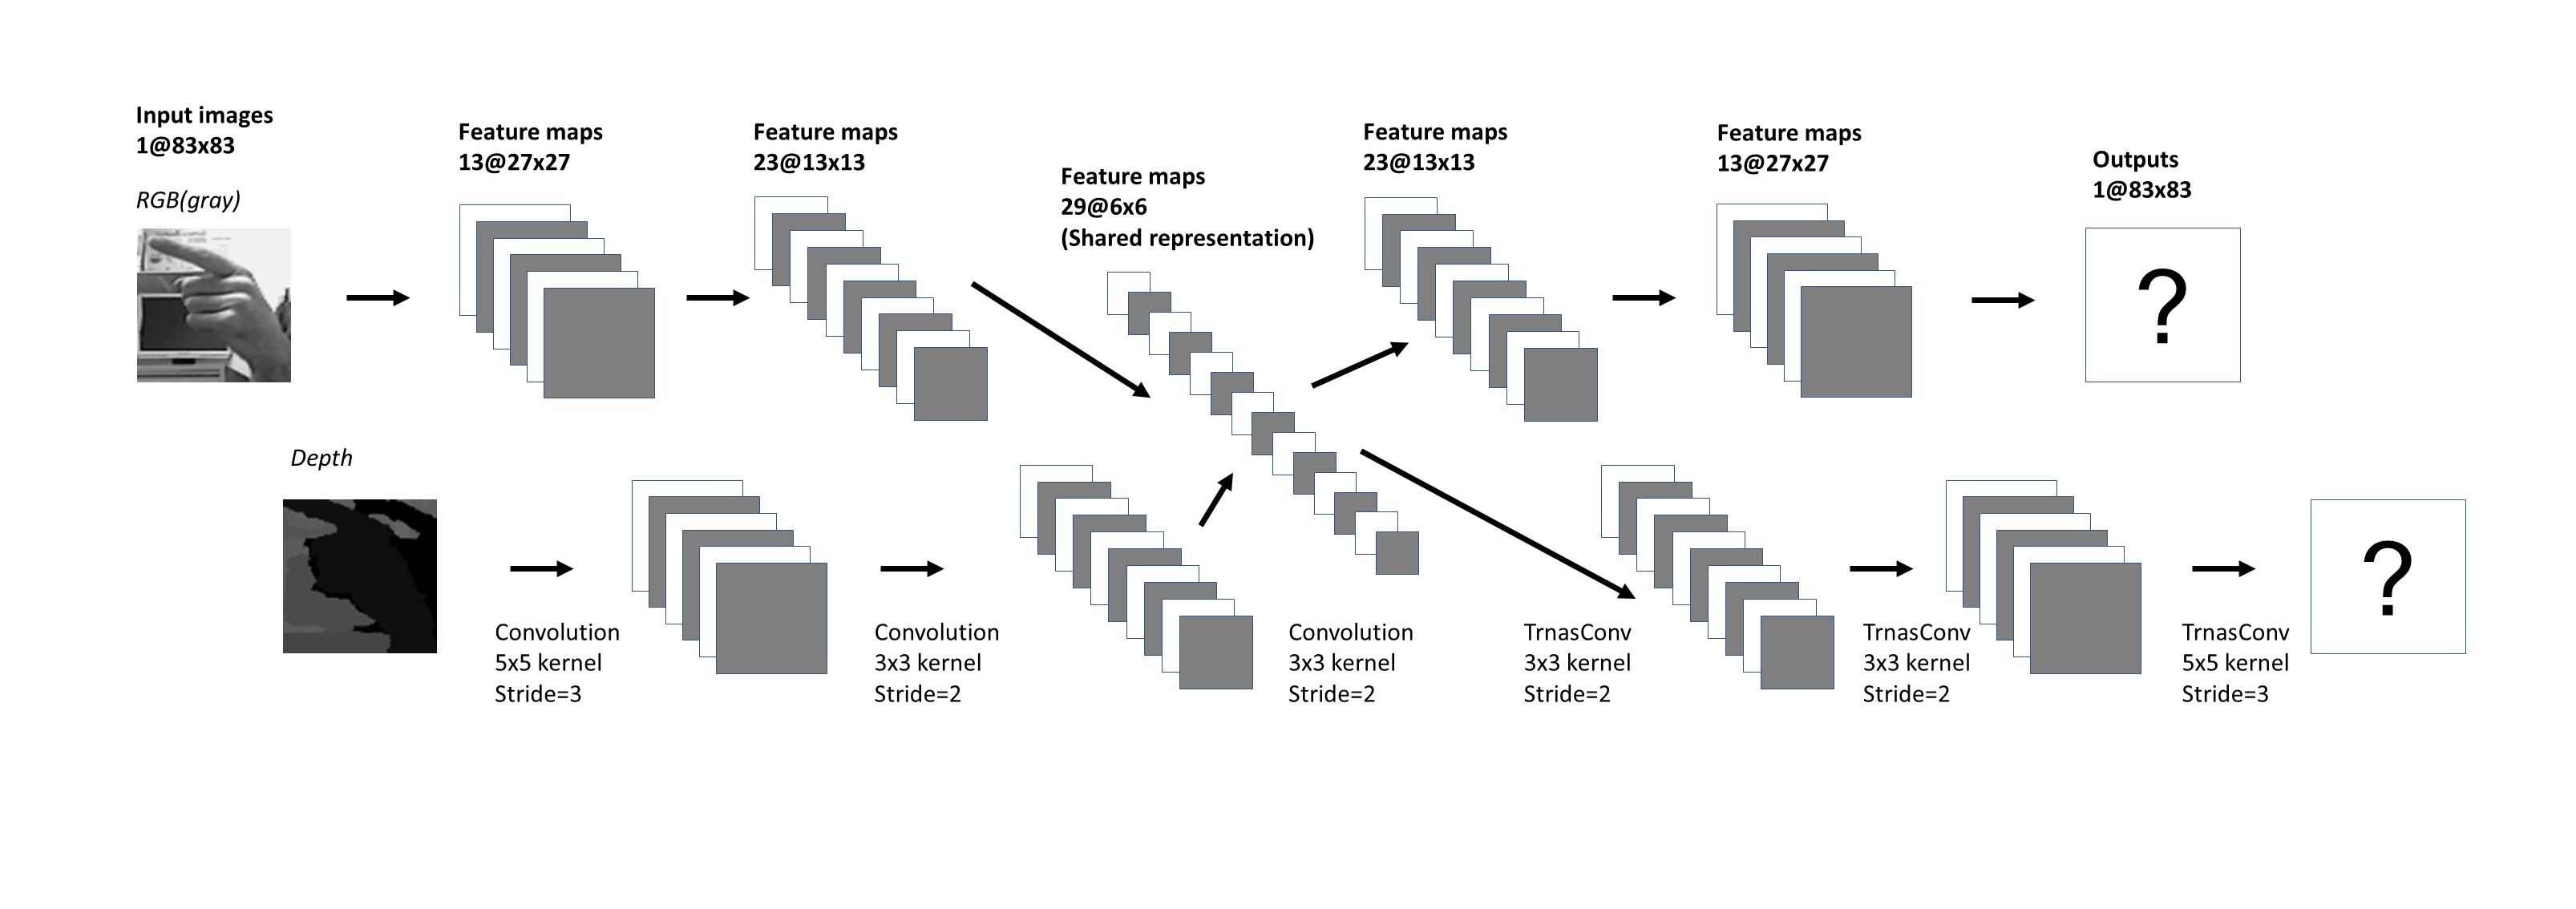
\includegraphics[width=0.95\linewidth]{architectures/FAE5}
  \caption{%
    \textbf{The bimodal convolutional auto-encoder model that is
      used to learn shared multimodal representation.}\\[0.1em]
    We simply take the CAE architecture that is introduced
      \autoref{fig:CAE5} for each modaliy but force them to have a
      shared middle layer by adding the corresponding activation values.
      We then try to reconstruct the two images separately through
      two disjoint paths. During training, I used $\alpha_0=0.01$,
      $\gamma = 0.8$ and $\lambda = 0.0004$ (see the first paragraph
      of section \ref{section:exp}) for the presented results.}
  \label{fig:FAE5}
\end{figure}

To prevent the network from finding representations such that different
hidden units are tuned for different modalities separately, random
dropouts are added to inputs. I first draw a random number $p$ between
0 and 1. Each pixel of the color modality is then kept with probability $p$
while for the depth modality they're kept with probability $1-p$.
In particular, sometimes one modality can be totally absent whereas
the whole clean image is given for the other modality.
In this way I gaurauntee also that I always have enough information
in input for the reconstruction if the two modalities are
used jointly by the network.
In addition, proper scaling were considered to keep the expected
sum of the activations at each layer to be the same.

Ideally, we expect that the network is able to capture correlations
across different modalities and learn a better single modality
representation thanks to the presence of the other modality
during feature learning. To verify this hypothesis, I built a perceptron
on the top of the middle layer of the architecture and trained it
in a supervised way while only one modality was given in input. For example,
if I wanted to train a classifier for color images, zeros were fed as
depth inputs.

The results are shown in \autoref{tab:ASL_classif}.
We can observe an improvement of the classification accuracy for a
classifier that is based on the learned shared representation 
compared to the one that is built on the features that are learned by
an unimodal CAE. This reveals the uitiliy of using multiple modalities
for representation learning. However, more tests and statistics
are necessary for validating this preliminary result.

How about exploiting the information from the two modalities in a
totally supervised way? I took the CNN architecture of \autoref{fig:CNN10}
for color and depth images separately until the seventh layer where
a fusion was carried out. After training the network, the prediction
accuracy was always at about 80\% and no improvement was obtained compared
with a CNN trained only on color inputs. The little or no improvement
may be due to the similarity between the two modalities. Supposing that
color images contain already all the necessary information for the task
at hand, then depth maps would not bring any supplementary information
that benefits the specific purpose I defined. Again, still more tests,
and perhaps with different data, are needed to verify this hypothesis.

There is yet another interesting result that's worth mentioning.
In an experiment, I trained a CAE (the setting presented in
\autoref{fig:CAE5}) for noisy depth inputs but instead of comparing
the outputs with clean depth images they're compared with clean
color images. In other words, I tried to construct the color modality from
noisy depth maps. When I did the classification based on the learned
representation, the performance was comparable with the perceptron
that was built on the CAE features that were learned by a normal
depth CAE. This is particularly useful when one or several
modalities are noisy whereas clean information are available for the others.

\begin{table}[H]
  \tabcolsep = 9pt
  \caption{\textbf{Classification performance on the ASL Finger Spelling
    dataset}\\[0.1em]
    Raw) Perceptron that reads raw input data.\\[0.1em]
    CAE features) Perceptron stacked on the middle layer of the CAE.
      (\autoref{fig:CAE5} and \ref{subsection:CAE}).\\[0.1em]
    Shared) Perceptron that exploits the shared representation learned
      by a bimodal CAE (\autoref{fig:FAE5} and
      \ref{subsection:shared}).\\[0.1em]
    CAE architecture) Perceptron stacked on the middle layer of the CAE
      but train the whole network in a supervised way as a CNN.
      (\autoref{fig:CAE5} and \ref{subsection:CAE}).\\[0.1em]
    CNN) The CNN architecture in \autoref{fig:CNN10}
      (\autoref{fig:CNN10} and \ref{subsubsection:ASL_CNN}). \\[0.1em]
    The used hyperparameters are $\alpha_0=0.005$, $\gamma=0.8$ and
    $\lambda=0.0004$ (see the first paragraph of section \ref{section:exp}).
    We notice that we have exactly the same network
    architecture for the middle three exerimental setups and only the
    training process differs one from another.
    }
  \label{tab:ASL_classif}
  \begin{tabular*}{\linewidth}{>{\bf}llccccc}
    \toprule
    && Raw & CAE features & Shared & CAE architecture & CNN\\
    \midrule
    \multirow{2}{*}{Intensity} &
    train & 69.47 \% & 78.87 \% & 85.85 \% & 91.29 \% & 99.69 \% \\
    & test & 32.64 \% & 50.24 \% & 53.38 \% & 65.44 \% & 79.73 \% \\
    \midrule
    \multirow{2}{*}{Depth} &
    train & 63.64 \% & 79.61 \% & 81.83 \% & 88.80 \% & 97.24 \% \\
    & test & 29.93 \% & 41.64 \% & 42.85 \% & 55.62 \% & 64.46 \% \\
    \bottomrule
  \end{tabular*}
\end{table}
\vspace{-10pt}

We may also want to ask if this architecture, when a partial input with
only one modality is given, is able to infer the values of the missing
modality.
Several examples can be seen in \autoref{fig:color_depth_restoration}.
Visually speaking, the reconstruction result seems better when
both modalities are available in input even though they're both very noisy.

\begin{figure}[H]
  \centering
  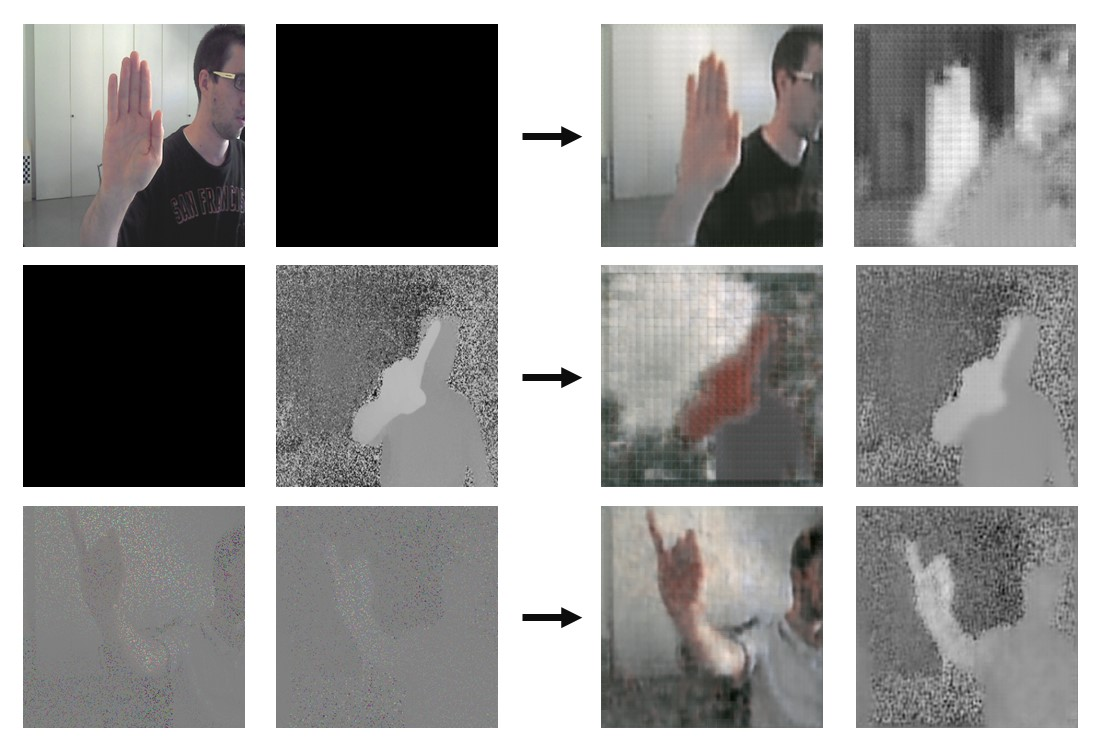
\includegraphics[width=\linewidth]{dataset/senz3d/reconstructions}
  \caption{%
    \textbf{Restore color and depth images from incomplete input
      information.}\\[0.1em]
    Top) Only the color image is given.\\[0.1em]
    Middle) Only the depth image is given.\\[0.1em]
    Botttom) Both modalities are given but with little information
      (10\% of pixels).\\[0.1em]
    From left to right: original images $\rightarrow$ images with
      dropout $\rightarrow$ reconstructed images.
    }
  \label{fig:color_depth_restoration}
\end{figure}

\subsection{Transfer learning} \label{subsection:AVSR_transfer}

In real world, we face frequently an imbalance in the amount of data
among different modalities, and acquiring a parallel multimodal
dataset is extremely resource consuming.
The same defect equally exists for an autonomous robot because
multimodal information received by its different sensors are not always
related.
Consequently, I'll discuss the knowledge transfer problem between
different modalities in the second part of this section.
The goal is exploit information from one modality to improve the
learning of another modality.
This work is very similar to what is done in \cite{S. Moon 2015},
but at the same time it can also be viewed as a form of zero-shot
learning \cite{A. Frome 2013, R. Socher 2013} since as we will see,
not every label used for testing is directly presented during training.

I studied particularly the transfer between speech and lip-reading
video data using the AVLetters dataset. First the dataset was separated
randomly into two training and test set.
They are respectively noted $Tr$ and $Te$.
$Tr$ contained 600 data samples while $Te$ comprised the left 180 instances.
For $X$ an arbitrary subset of data, $X^a$ and $X^v$ denote respectively
the audio and video data in $X$.

\begin{figure}[!b]
  \centering
  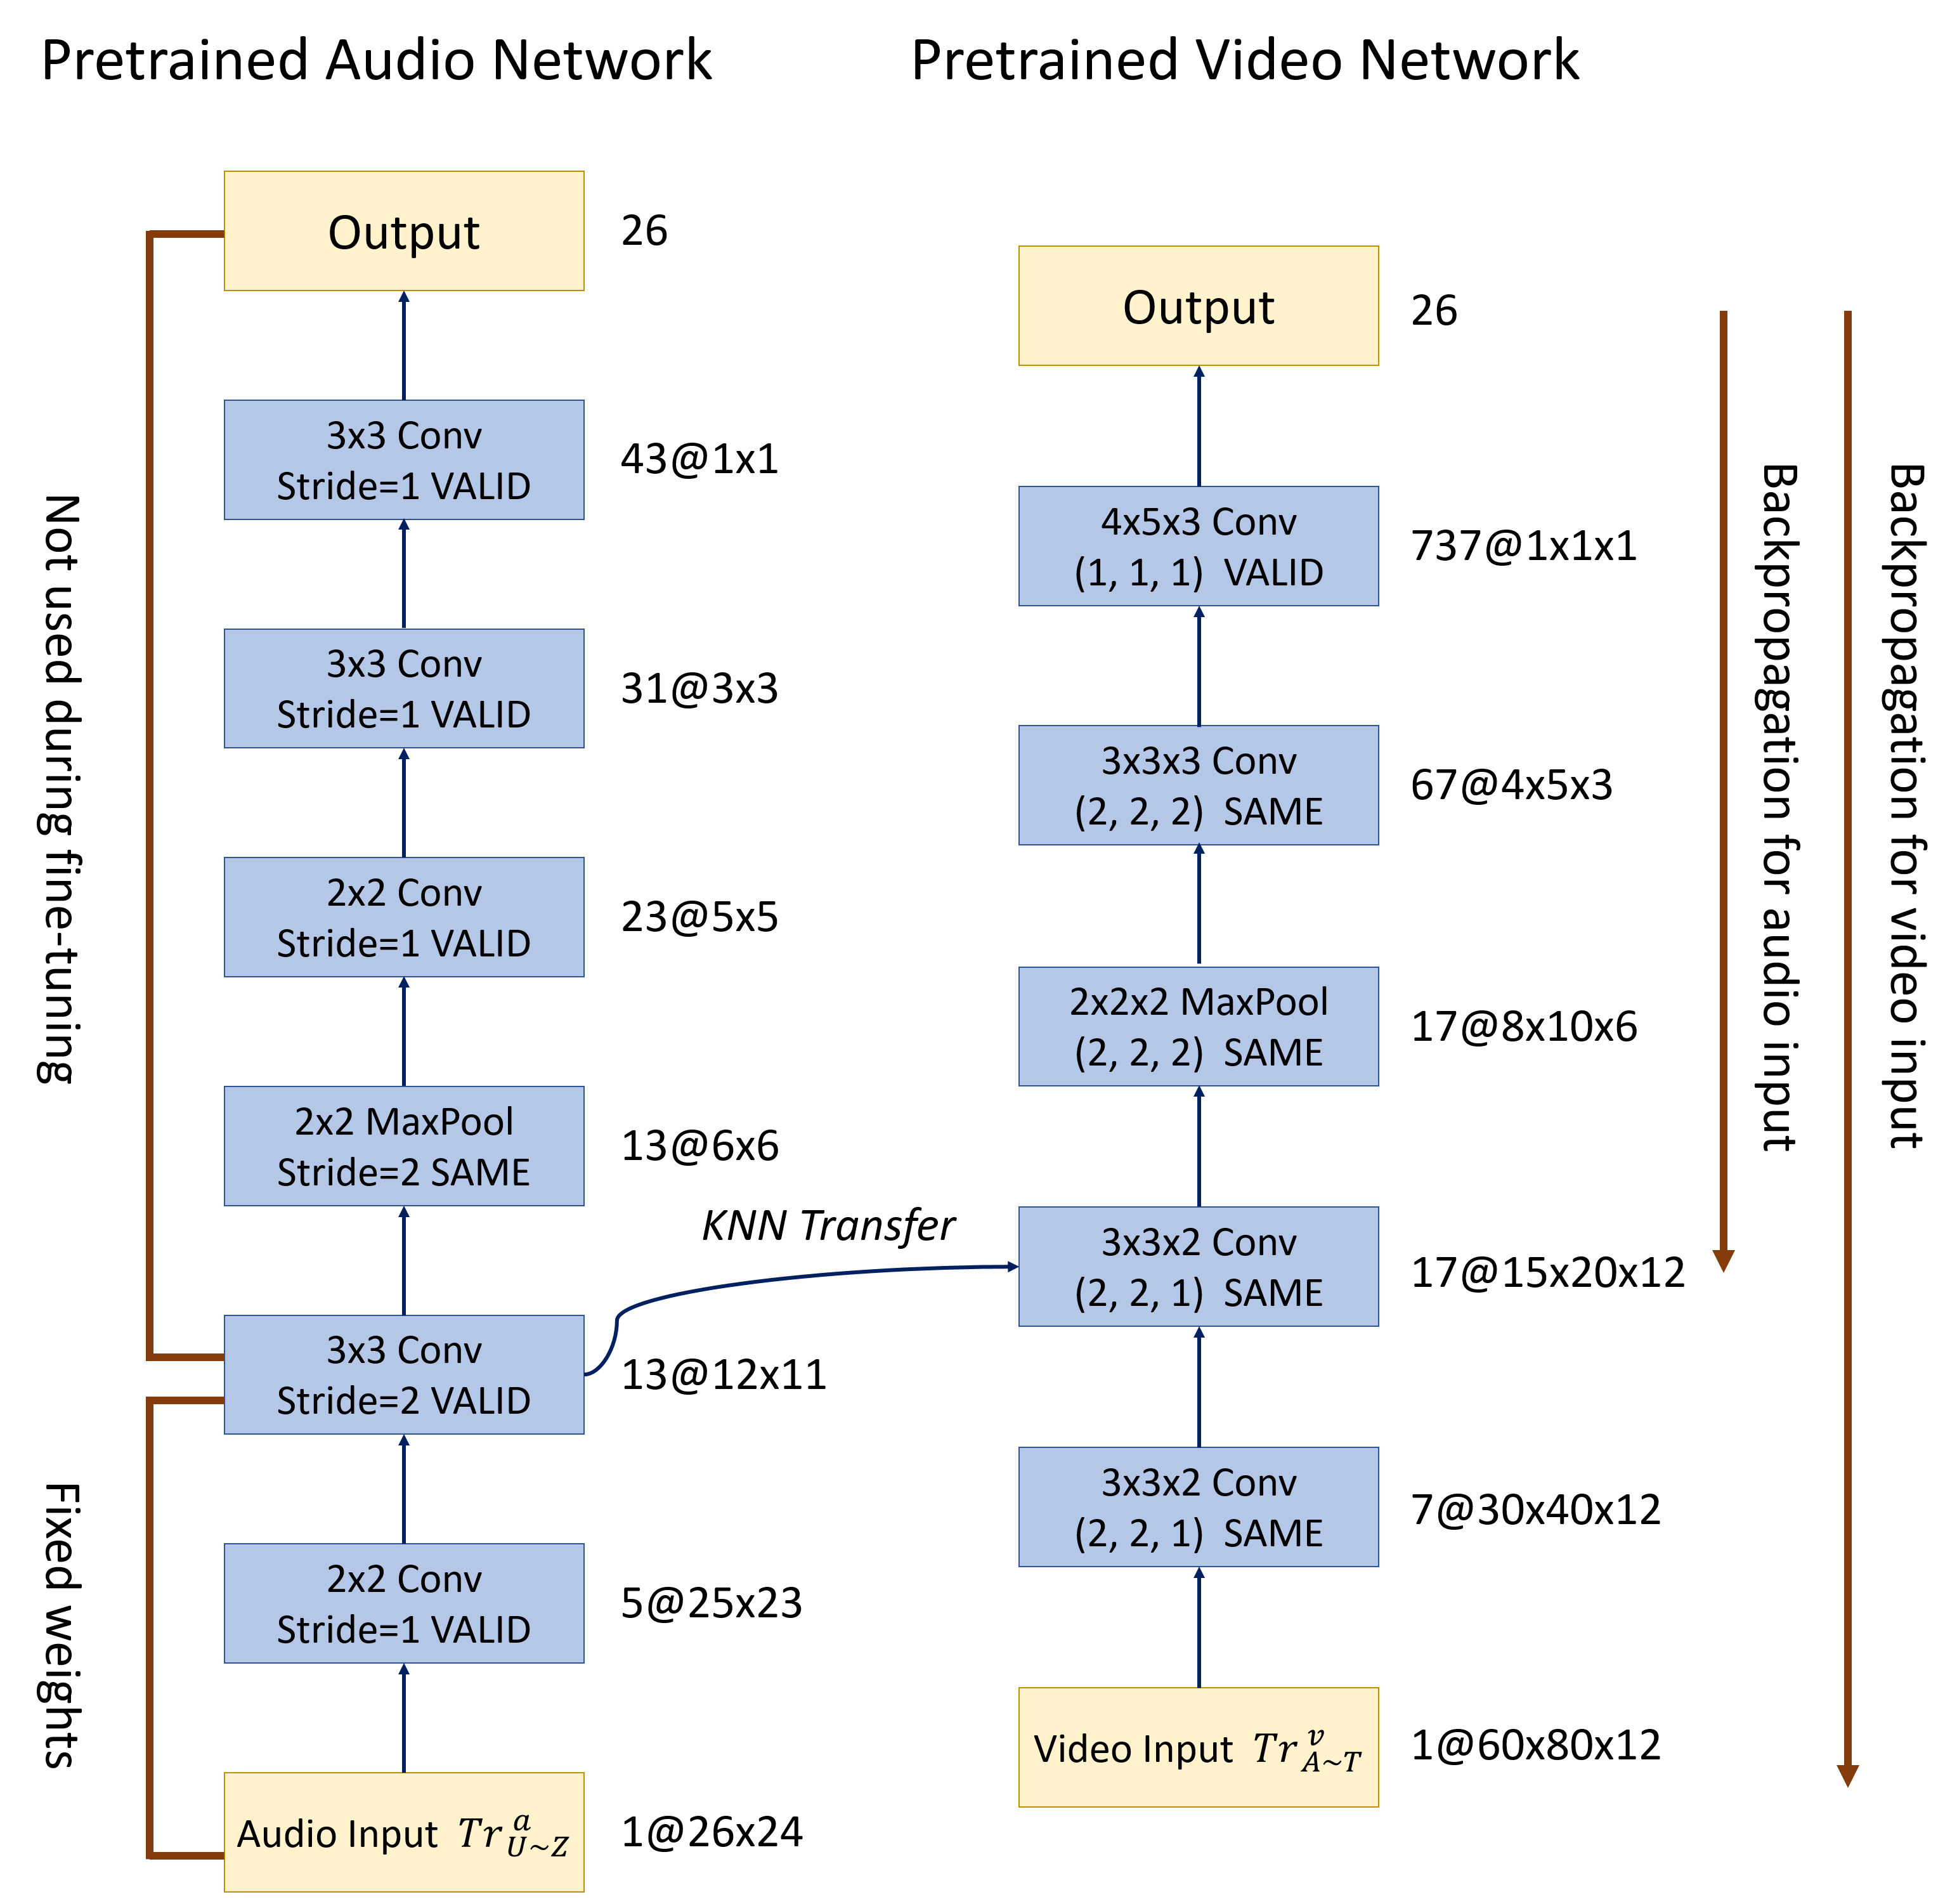
\includegraphics[width=0.9\linewidth]{architectures/AVSR_transfer}
  \caption{%
    \textbf{Illustration of the transfer learning approach applied in
      audio and lip-reading speech recognition tasks.}\\[0.1em]
    We first learn two separated models for audio and visual inputs
      (in my case two CNNs) and try to fine-tune the video network
      with transferred audio data.
    }
  \label{fig:AVSR_transfer}
\end{figure}

Next, to simulate the imbalance of data quantity between different
modalities in the real world, I further splitted $Tr$, $Te$ into
$Tr_{A\sim T}$, $Tr_{U\sim Z}$, $Te_{A\sim T}$ and $Te_{U\sim Z}$
according to the label of each sample.
For instance, a lip-reading video of a speaker saying E is in either
$Tr_{A\sim T}^v$ or $Te_{A\sim T}^v$.
During the first training stage, the video model was only accessible
to a partial label space. The network (see \autoref{fig:AVSR_transfer}
and \autoref{tab:AVSR_transfer} for archticture and hyperparameters)
was trained on $Tr_{A\sim T}^v$ which contained 466 samples.
On the other hand, the audio model was trained on the whole
label space $Tr^a$.

After that, I wanted to leverage speech data to fine-tune the network
trained for video recognition. For a data sample $x^a\in Tr_{U\sim Z}^a$,
I first computed its audio representation $h^a(x^a)$ that was taken from
some hidden layer of audio model. A transfer function $\mathcal{T}$ was used
to approximate the video representation of this data sample.
That is, we want $\mathcal{T}(h^a(x^a))\approx h^v(x^v)$. Finally, I
fine-tuned the subnetwork situated after the hidden video layer that
was taken as representation via a standard backpropagation algorithm.
I chose audio as the source modality for two principal reasons.
First, generally the quantity of audio data surpasses that of visual
data. Second, the lip-reading task generally appears to be more
difficult than that of audio speech recognition.

The detailed experiment is presented in \autoref{fig:AVSR_transfer}.
For both audio and video network I choose the second hidden layer for
transfer. For the sake of simplicity, an instance-based approach
(KNN-based mapping) was employed to define $\mathcal{T}$.
I obtained mapping of a new audio
input $x^v$ by first finding the $K$-closest audio samples of
$Tr_{A\sim T}^a$ in the representation space, and then returning the
average values of the corresponding video samples
(also in the representation space).

Nonetheless, if only audio inputs were presented during fine-tuning, it
might cause a bias of the fine-tuned network towards the six new classes.
To avoid this problem, data from $Tr_{A\sim T}^v$ were also fed as input
from time to time to fine-tune the whole network. Concretely, with
probability $p_a$ audio data was presented and otherwise video input
was given. At the end, the new network was tested on different parts of
video data (e.g. $Tr_{A\sim T}^v$ and $Te_{U\sim Z}^v$) for evaluataion.

Many experiments with various hyperparameter values were conducted
and some results are shown in \autoref{tab:AVSR_transfer}.
We see that despite the fact that the overall performance is not certainly
improved by knowledge transfer,
the fine-tuned network is now able to classify
samples whose labels range from U to Z with an accuracy of 10-20\%
(\textbf{Exp1}, 21.64\% for $Tr_{U\sim Z}^v$ and 15.22\% for
$Te_{U\sim Z}^v$). It shows the utility of the transfer learning approach
which enables us to classify labels that are not at all available
for the target modality.
During fine-tuning, the magnitude of learning rate is equally important.
As we can see, if the learning rate is too high, it can deteriorate
the pre-trained network and the performance may drop drastically
(\textbf{Exp2}).
On the other hand, as predicted before, if only audio data labeled from
U to Z are provided for fine-tuining, the classification performance
drops for the first twenty labels even though a higher accuracy
can be achieved for the last six labels (\textbf{Exp3}, 45.52\% for
$Tr_{U\sim Z}^v$ and 41.34\% for $Te_{U\sim Z}^v$).

\begin{table}[H]
  \tabcolsep = 13pt
  \caption{\textbf{Some results of the audio-visual transfer experiment.}
    \\[0.1em]
  The audio model was pre-trained with $\lambda=0.1$, $\alpha_0=0.005$ and
  $\gamma=0.8$ while the video model was pre-trained with $\lambda=0.0004$,
  $\alpha_0=0.002$ and $\gamma=0.96$. The transfer learning experiment
  was carried out under the setting $\lambda=0.0004$, $\gamma=0.8$, $K=12$
  and was trained for 160 steps.
  For \textbf{Exp1}, \textbf{Exp2} and \textbf{Exp3}, I used respectively
  $\alpha_0 = 0.001, 0.005, 0.001$ and $p_a = 0.85, 0.85, 1$.\\[0.1em]
  For the meaning of different variables see the first paragraph of
  section \ref{section:exp} and also the text of
  \ref{subsection:AVSR_transfer}.
  Notice that since $p_a = 1$ for \textbf{Exp3} no visual input is given
  in input during fine-tuning.
  }
  \label{tab:AVSR_transfer}
  \begin{tabular*}{\linewidth}{>{\bf}lcccccc}
    \toprule
    & $Tr^v$ & $Tr^v_{A\sim T}$ & $Tr^v_{U\sim Z}$
    & $Te^v$ & $Te^v_{A\sim T}$ & $Te^v_{U\sim Z}$\\
    \midrule
    No transfer & 77.67 \% & \textbf{100} \% & 0 \% & \textbf{40.56} \%
    & \textbf{54.48} \% & 0 \% \\
    Exp1 & \textbf{81.17} \% & 98.28 \% & 21.64 \% & 39.44 \%
    & 47.76 \% & 15.22 \% \\
    Exp2 &  40.83 \% & 51.07 \% & 5.22 \% & 23.89 \%
    & 30.60 \% & 4.35 \% \\
    Exp3 & 19.67 \% & 12.23 \% & \textbf{45.52} \% & 12.22 \%
    & 2.24 \% & \textbf{41.34} \% \\
    \bottomrule
  \end{tabular*}
\end{table}
\vspace{-1em}

\section{Conclusion and Perspectives} \label{section:conclusion}

In this report, I studied two different multimodal learning
architectures and evaluated them on three different datasets.
Several preliminary results were obtained and my work ensured the
possiblity and the possible benefit of taking into multiple modalities
into account while dealing with real world problems.
To go further in this direction, my work can be improved in several ways.
First, datasets with bigger size and higher variety should give more
reliable results.
Second, a more exhaustive search of hyperparameters may lead to better
outcomes. Finally, we should also pay attention on the modalities
that we deal with and if the adopted method is really appropriate.

Ideally, we want to apply these techniques to real
data coming from human-robot interactions. In this way, we may be able to
improve the perception of the robot thanks to the presence of
multiple sensors. Learning the shared representation in a totally
unsupervised way can be useful for the development of an autonomous
robot and absence of constant relation between different modalities
can be compensate by the knowledge transfer approach.
